\documentclass[12pt]{article}
\usepackage[margin=1in]{geometry}
\usepackage{amsmath,amssymb,amsthm}
\usepackage{tikz}

\setlength{\parindent}{0pt}
\setlength{\parskip}{0.8em}

\begin{document}

\begin{center}
{\large\bfseries MATH 5810 Spring 2026\\Homework 3}
\end{center}

\medskip

Undergraduate students must submit solutions for any six problems from $1-8$, and one of $9, 10$.\\
Graduate students must submit the solutions for all problems.

\noindent\rule{\textwidth}{0.8pt}

\begin{center}
{\large\bfseries\color{red} Graph Coloring}
\end{center}

\textbf{1)} Prove that the \underline{edge} chromatic number of every regular bipartite graph $G$ is equal to $\Delta(G)$.

\medskip

\textit{Hint: You may use the fact that every regular bipartite graph has a perfect matching (this was proved in class earlier).}

\medskip

\begin{proof}
Let $G$ be a regular bipartite graph where every vertex has degree $n$, so that $\Delta(G) = n$. We proceed by induction on $n$.

\textbf{Base case:} If $n = 1$, then $G$ is a perfect matching and all edges can be colored with a single color, so $\chi'(G) = 1 = \Delta(G)$.

\textbf{Inductive step:} Assume the result holds for all regular bipartite graphs with maximum degree $n - 1$. Since $G$ is an $n$-regular bipartite graph, by the theorem proved in class, $G$ has a perfect matching $M$. The edges of $M$ are pairwise non-adjacent, so we may assign them all the same color, say color $1$.

Now consider the graph $G' = G - M$ obtained by removing the edges of $M$. Since every vertex in $G$ was incident to exactly one edge of $M$, every vertex in $G'$ has degree $n - 1$. Moreover, $G'$ is still bipartite (with the same bipartition as $G$). Thus $G'$ is an $(n-1)$-regular bipartite graph.

By the inductive hypothesis, $\chi'(G') = n - 1$, so the edges of $G'$ can be properly colored with $n - 1$ colors. Together with the color used for $M$, we obtain a proper edge coloring of $G$ using $n$ colors. Therefore $\chi'(G) \leq n = \Delta(G)$.

Since $\chi'(G) \geq \Delta(G)$ for any graph (every edge incident to a vertex of maximum degree must receive a distinct color), we conclude $\chi'(G) = \Delta(G)$.
\end{proof}

\textbf{2)} Prove that if $G$ is a regular graph on odd number of vertices, then the \underline{edge} chromatic number of $G$ is $\Delta(G)+1$.

\medskip

\begin{proof}
Let $G$ be a $k$-regular graph on $n$ vertices where $n$ is odd. Note that by the handshaking lemma, $kn = 2|E(G)|$, so $k$ must be even since $n$ is odd. Write $k = \Delta(G)$.

\textbf{Lower bound} ($\chi'(G) \geq k + 1$): Suppose for contradiction that $\chi'(G) = k$, i.e., the edges of $G$ can be properly colored with $k$ colors. Since $G$ is $k$-regular, every vertex is incident to $k$ edges, all of which must receive distinct colors. Thus every vertex is incident to an edge of every color. This means each color class (the set of edges sharing a color) covers every vertex --- that is, each color class is a perfect matching. But $n$ is odd, so no perfect matching exists. Contradiction. Therefore $\chi'(G) \geq k + 1$.

\textbf{Upper bound} ($\chi'(G) \leq k + 1$): This follows from Vizing's Theorem, which states that for any simple graph $G$,
\[\Delta(G) \leq \chi'(G) \leq \Delta(G) + 1.\]
Therefore $\chi'(G) = k + 1 = \Delta(G) + 1$.
\end{proof}

\textbf{3)} Show that if $G$ has a vertex $v$ with $\deg_G(v) < \Delta(G)$, then $\chi(G) \leq \Delta(G)$.

\medskip

\textit{Hint: use a spanning tree to order the vertices in such a way that the greedy algorithm will use at most $\Delta(G)$ colors.}

\medskip

\begin{proof}
Let $G$ be a graph with $\Delta(G) = \Delta$, and let $v$ be a vertex with $\deg_G(v) < \Delta$. Let $T$ be a spanning tree of $G$ rooted at $v$.

Order the vertices $v_1, v_2, \ldots, v_n$ so that leaves of $T$ come first and the root $v$ comes last. Specifically, use a reverse breadth-first search ordering: vertices at the greatest depth in $T$ are listed first, and $v = v_n$ is listed last. (Within the same depth level, the order is arbitrary.)

We apply the greedy coloring algorithm with a palette of $\Delta$ colors, coloring vertices in the order $v_1, v_2, \ldots, v_n$.

\textbf{Non-root vertices:} Consider any vertex $v_i \neq v$. In the spanning tree $T$, the parent of $v_i$ (its neighbor on the path toward the root $v$) appears later in the ordering, so it is uncolored when we color $v_i$. Thus, at most $\deg_G(v_i) - 1 \leq \Delta - 1$ of $v_i$'s neighbors in $G$ are already colored. Since we have $\Delta$ colors available, at least one color is unused among $v_i$'s colored neighbors, and the greedy algorithm assigns it.

\textbf{Root vertex:} When we color $v = v_n$ last, all of its neighbors in $G$ may already be colored. However, $\deg_G(v) < \Delta$, so $v$ has at most $\Delta - 1$ neighbors. Therefore, at most $\Delta - 1$ colors appear among its neighbors, and at least one of the $\Delta$ colors remains available.

In both cases, the greedy algorithm never requires more than $\Delta$ colors. Therefore $\chi(G) \leq \Delta(G)$.
\end{proof}

\textbf{4)} Show that every $k$-chromatic graph $G$ has at least $\binom{k}{2}$ edges.

\begin{center}
{\large\bfseries\color{red} Planar Graphs}
\end{center}

\textbf{5)}

\begin{center}
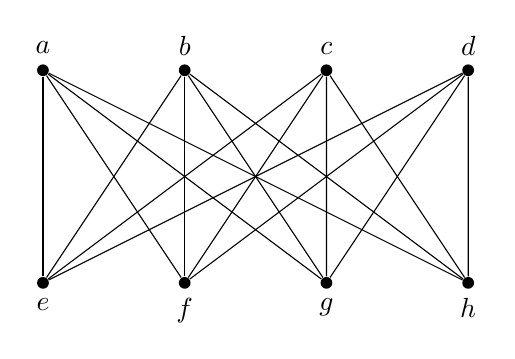
\begin{tikzpicture}[scale=1.8, every node/.style={circle, fill=black, inner sep=1.5pt}]
  \node[label=above:$a$] (a) at (0,1.5) {};
  \node[label=above:$b$] (b) at (1,1.5) {};
  \node[label=above:$c$] (c) at (2,1.5) {};
  \node[label=above:$d$] (d) at (3,1.5) {};
  \node[label=below:$e$] (e) at (0,0) {};
  \node[label=below:$f$] (f) at (1,0) {};
  \node[label=below:$g$] (g) at (2,0) {};
  \node[label=below:$h$] (h) at (3,0) {};
  \foreach \i in {a,b,c,d}
    \foreach \j in {e,f,g,h}
      \draw (\i) -- (\j);
\end{tikzpicture}
\end{center}

\begin{enumerate}
\item[a)] Show that the graph above is planar by redrawing it as plane graph and then verify the Euler's formula for the plane graph.

\item[b)] The Euler's Formula for connected graphs says that
\[n - m + f = 2\]
where $n, m, f$ are the number of vertices, edges and faces respectively. Extend this formula to all graphs by showing that
\[n - m + f = k + 1\]
where $k$ is the number of connected components.
\end{enumerate}

\textbf{6)} Let $G$ be a simple planar graph.

\begin{enumerate}
\item[a)] Show that $G$ has a vertex $v$ with degree less than 6. (\textit{Hint: use the bound $m \leq 3n - 6$ proved in class.})

\item[b)] Show that $\chi(G) \leq 6$. (\textit{Hint: use part (a) and induction.})
\end{enumerate}

\textbf{7)} Let $G$ be a simple graph.

\begin{enumerate}
\item[b)] Prove that if $G$ has at least 11 vertices, then either $G$ or its complement $\overline{G}$ must be nonplanar.

\textit{Hint: you may use the result $m \leq 3n - 6$ that we proved in class.}
\end{enumerate}

\textbf{8)} Let $G$ be a \underline{simple connected} planar graph.

\begin{enumerate}
\item[a)] Prove that if $G$ has less than 12 vertices, then $G$ has a vertex of degree at most 4.

\textit{Hint: you may use the result $m \leq 3n - 6$ that we proved in class.}

\item[b)] Prove that if $G$ has less than 30 edges, then $G$ has a vertex of degree at most 4.

\textit{Hint: you may use part (a) to prove part (b).}
\end{enumerate}

\begin{center}
{\large\bfseries\color{red} Line Graphs}
\end{center}

\textbf{9)} Let $L(G)$ be the line graph of $G$.\\
\hspace*{1.5em}Prove that $G \cong L(G)$ if and only if $G$ is 2-regular.

\begin{center}
{\large\bfseries\color{red} Connectivity}
\end{center}

\textbf{10)} Let $\kappa(G)$ be the vertex connectivity and $\lambda(G)$ be the edge connectivity of $G$.

\begin{enumerate}
\item[a)] Prove that $\kappa(G) \leq \lambda(G)$.

\item[b)] Show that the difference between $\kappa(G)$ and $\lambda(G)$ can be arbitrarily large.\\
(i.e., for any given $r \in \mathbb{Z}^+$, construct a graph $G$ with $\lambda(G) - \kappa(G) = r$).
\end{enumerate}

\end{document}
